\chapter{Harmonic Beacon: The Experiential Probe}

\epigraph{\emph{It is not a sound object. It is a field.}}{}



\section{What the Harmonic Beacon is}


If Chapter 11 asked what becomes visible when harmonic hypotheses are made computational, this chapter asks what becomes visible when they are made physical, acoustic, and experiential. The Beacon is the experiential probe of HIT. It is a device built to generate a sustained harmonic field rather than an isolated sound event, and to do so under conditions precise enough that the resulting field can be treated as an object of investigation rather than as an atmospheric effect.

That distinction matters from the start. The Beacon is not a metronome, because its point is not periodic marking. It is not a drone, because the field it produces is internally structured rather than spectrally flat. It is not a sound bath, because its organizing principle is not immersion alone but sustained harmonic proportion. A motor excites a string continuously, and the instrument holds open a dense pattern of interacting partials that would otherwise collapse as soon as the note decayed. What the listener encounters is not a single pitch extended in time but a living interference field.

Operationally, the Beacon begins with a resonant source, an excitation method, a tuning procedure, and a room. In the earliest configuration the source is a guitar string coupled to a resonant body, and the excitation is a motor that keeps the system vibrating continuously instead of allowing a plucked event to die away. Later generations replace or complement that source with tuning forks, piezoelectric actuators, oscillator banks, and live networked outputs, but the logic remains the same. A harmonic field is sustained, tuned by coherence of the resulting interference pattern, and then probed through listening, biosignal capture, or visible pattern formation. The object of study is therefore not a recorded sound file. It is a physically maintained acoustic condition.

The reports surrounding that field are strikingly consistent. Listeners speak of melodies, choral textures, bagpipes, voices, and other organized sounds that are not explicitly present in the source. The useful term here is harmonic pareidolia. The point is to treat those perceptions as situated readings that emerge within a highly structured acoustic field rather than as a single fixed content that the source would simply contain in advance. The field is structured enough to sustain recognition and open enough to remain underdetermined.

That is why the Beacon matters for HIT. It provides a controllable source of natural harmonic organization in a register that computation alone cannot settle: embodied exposure to a sustained acoustic field. Phideus can test what ratio-guided structure does inside representation. The Beacon tests what a harmonic field does when it occupies a room, meets a body, and becomes part of an experienced environment. The chapter that follows is therefore not about a device in isolation. It is about the construction of an instrument through which the theory can be probed in physiological and experiential terms.

\begin{figure}[ht]
\centering
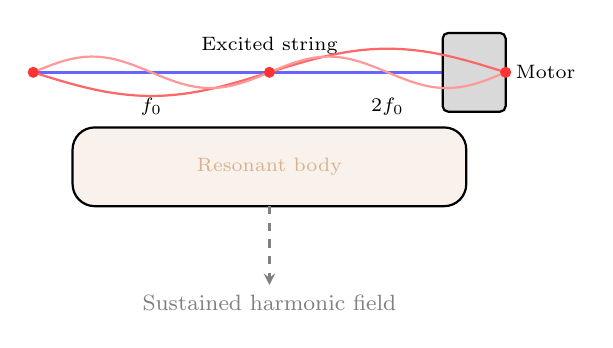
\begin{tikzpicture}[
    >=stealth, thick,
    every node/.style={font=\footnotesize}
]
% Guitar body outline (simplified)
\draw[rounded corners=8pt, fill=brown!10] (-2.5, -0.5) rectangle (2.5, 0.5);
\node[font=\scriptsize, text=brown!60] at (0, 0) {Resonant body};

% String
\draw[very thick, blue!60] (-3, 1.2) -- (3, 1.2);
\node[font=\scriptsize, above] at (0, 1.3) {Excited string};

% Motor
\draw[fill=gray!30, rounded corners=2pt] (2.2, 0.7) rectangle (3.0, 1.7);
\node[font=\scriptsize, right] at (3.0, 1.2) {Motor};

% Standing wave pattern
\draw[red!60, thick, samples=100, domain=-3:3] plot (\x, {1.2 + 0.3*sin(180*\x/3)});
\draw[red!40, thick, samples=100, domain=-3:3] plot (\x, {1.2 + 0.2*sin(360*\x/3)});

% Nodes
\foreach \x in {-3, 0, 3} {
    \fill[red!80] (\x, 1.2) circle (2pt);
}

% Labels
\node[font=\scriptsize, below] at (-1.5, 1.0) {$f_0$};
\node[font=\scriptsize, below] at (1.5, 1.0) {$2f_0$};

% Arrow: sound field
\draw[->, dashed, gray] (0, -0.5) -- (0, -1.5) node[below] {Sustained harmonic field};
\end{tikzpicture}
\caption{Schematic of the Beacon Guitar (first generation). A motor continuously excites a string coupled to a resonant body, sustaining a dense interference field of interacting partials rather than a decaying plucked event. Harmonic nodes are marked along the string.}
\label{fig:beacon_device}
\end{figure}


\section{Principle of operation: the harmonic gravitational field}


The Beacon is physically simple and experimentally demanding. A string under continuous excitation does not present only a fundamental. It presents the full harmonic series at once, with amplitudes and beat patterns shaped by the material properties of the string, the excitation point, the resonant body, and the room in which the instrument sounds. Classical acoustics has long treated that problem as one of coupled source, resonator, and field rather than isolated pitch production \parencite{rayleigh_1877, benade_1973, fletcher_1996}. The motor's function is not decorative automation. It converts an event that would normally decay into a sustained field in which the interaction among partials can be held open long enough to become perceptible, measurable, and tunable.

At the most compressed level, the harmonic logic can be written as:

$$
f_n = n f_0
$$

and the resulting field as:

$$
s(t) = \sum_{n=1}^{N} A_n \cos(2 \pi n f_0 t + \phi_n)
$$

where the amplitudes and phases are shaped by the source, the excitation geometry, the resonant body, and the room. The Beacon does not isolate one member of that series. It sustains a field in which several members remain simultaneously active and mutually constraining.

The central operation is therefore not "play a frequency" but stabilize a proportional field. Tuning is not performed by matching the system to an abstract external standard. It is performed by moving the excitation until the interference pattern becomes maximally coherent. In practice that coherence can be checked by ear, by laser, or by cymatic visualization. The criterion is not pitch purity in the narrow sense. It is the quality of the pattern generated by the interaction among partials.

That tuning operation can be written schematically as:

$$
\theta^* = \arg\max_{\theta} C(\theta)
$$

where $\theta$ stands for the tunable configuration of the setup and $C(\theta)$ stands for the coherence of the resulting pattern. The point of the formula is not to pretend that the Beacon already has a closed scalar metric for every installation. It is to make the operational criterion explicit: the target is the most coherent field the configuration can sustain, not the nearest approximation to an external equal-tempered pitch.

The metaphor of a harmonic gravitational field should be read in that concrete sense. When the system is near the right tuning, it does not merely sound different. It feels as if nearby organization is being pulled into a more stable relation. When the tuning drifts, the field becomes less inhabitable and the interference pattern loses coherence. The metaphor is useful because it captures a basin-of-attraction structure. The Beacon constructs a highly organized acoustic condition under which harmonic stability and instability can be experienced, interpreted, and worked with as differences in constraint.

That construction connects directly to earlier chapters. Chapter 4 described consonance as functional relation rather than isolated property. Chapter 8 described harmonic organization as a problem of efficient coordination under constraint. The Beacon translates those claims into a physical setup. It produces a field in which the difference between stable and unstable proportion is not only thinkable but experientially accessible.


The room is part of the experiment. The Beacon field interacts with surfaces, volume, air column, and placement. Each room produces a situated version of the field. That is not a flaw to be hidden but a feature to be handled. The Beacon is not a transparent playback device whose environment should be treated as negligible. It is a probe in which source and space co-produce the acoustic condition under study.


\section{Evolution of the device}


The Beacon did not appear as a finished object. It evolved through successive generations, each of which solved one operational problem and exposed another. That history matters because it shows that the device is not an aesthetic artifact but a chain of engineering responses to experimental constraints: how to sustain the field, how to tune it repeatably, how to transport it, how to connect it to sensors, and how to separate what belongs to harmonic organization from what belongs to the material support that produces it.

The first generation was the Beacon Guitar. Its problem was also its strength: how to obtain a dense, continuous, physically resonant harmonic field rather than a short acoustic event. The solution was a motor-driven string coupled to a resonant body and tuned manually until the interference pattern stabilized. A key step in that tuning procedure was measuring the spectral profile of the instrument itself---the characteristic timbre of the resonant body---and then tuning the strings to natural-ratio intervals derived from their relation to that spectral signature rather than to an external equal-tempered standard. This version established the phenomenon and made the field effect undeniable. It also had the highest spectral richness of the line. But it demanded daily precision, constant retuning, manual skill, and a favorable room. In other words, the generation that produced the strongest field was also the least portable and the least forgiving.

The second generation, the Pico Robot, answered that fragility by moving toward struck tuning forks and related resonant elements. The question here was no longer only how rich the field could be, but how repeatably it could be produced without the tuning burden of the guitar configuration. The gain was robustness, portability, and easier deployment. The cost was a narrower harmonic palette and a different phenomenological character. What was gained in stability was paid for in spectral density and in the open, flowing character of the original string-based field.

A particularly productive line of exploration across the second and third generations has been the systematic study of the relationships among the first five natural harmonics ($1\!:\!2\!:\!3\!:\!4\!:\!5$). These ratios define the densest region of simple-integer relations and have repeatedly yielded some of the clearest interference structures in our practical work. Within the range explored so far, the same region has also tended to generate the most stable and geometrically distinct Lissajous figures, which is why it has become a natural meeting point between the Beacon's acoustic work and the visible-pattern exploration described below. The cover image of this book is itself a Lissajous figure traced from the simultaneous resonance of these five harmonics.

The third generation moved toward digital control. Here the problem was no longer local fragility but limited programmability and limited coupling to external systems. The response took two complementary forms. On one side, a bank of harmonically organized oscillators controlled through OSC, including a grid of 64 harmonic pads and routable synthesis targets. On the other, the same 64-pad control surface driving piezoelectric actuators that excite metal reeds at independently controllable frequencies, connected wirelessly via Bluetooth. The first form is purely digital; the second recovers the physical resonance of earlier generations while gaining the programmability and repeatability of digital control. Both forms made exact recall, remote control, and sensor coupling much easier. They also opened a path toward harmonic feedback systems in which other data streams can modulate the field in real time. But the move reopened a different methodological question: how much of the Beacon's distinctive effect belongs to harmonic organization as such, and how much belongs to the material behavior of a physically resonant source such as a string, fork, or resonant cavity?

The fourth generation, still emergent, extends the Beacon toward distributed and networked operation. In this regime the point is not only to build one device that sounds in one room, but to make a live Beacon available through app-based access, remote listening, and later networks of synchronized devices. The explicit design choice is important: the app is not conceived as playback of a canned recording, but as access to a Beacon that is sounding in real time somewhere in the network. At that point the Beacon stops being only a local laboratory instrument and starts becoming a platform. Methodologically, this changes what can be transported, what can be personalized, and what kind of collective or environmental evidence the system can eventually seek.

\begin{table}[ht]
\centering
\caption{Beacon device generations: evolution from laboratory instrument to distributed platform.}
\label{tab:beacon_generations}
\footnotesize
\renewcommand{\arraystretch}{1.08}
\begin{tabularx}{\textwidth}{@{}P{0.14\textwidth}Y Y P{0.10\textwidth}P{0.13\textwidth}@{}}
\toprule
Generation & Physical source & Problem solved & Porta\-bility & Spectral richness \\
\midrule
Beacon Guitar & String + resonant body, continuous motor & Produces dense sustained field & Low & Highest \\
Pico Robot & Tuning forks + compact resonators & Improves robustness and portability & High & Medium \\
Digital/OSC & Oscillator bank / piezoelectric actuators + 64-pad harmonic control surface & Enables repeatability and sensor coupling & Very high & Controllable \\
App/\newline Distributed & Live remote Beacon node, streaming & Extends device into platform & Universal & Configur\-able \\
\bottomrule
\end{tabularx}
\renewcommand{\arraystretch}{1}
\end{table}

\begin{figure}[H]
\centering
\begin{subfigure}[b]{0.48\textwidth}
    \centering
    
\includegraphics[width=\textwidth, height=5.5cm, keepaspectratio]{Beacon1_para_libro.jpg}
    \caption{Beacon Guitar (1st gen). Motor-driven string coupled to acoustic body.}
    \label{fig:beacon1}
\end{subfigure}
\hfill
\begin{subfigure}[b]{0.48\textwidth}
    \centering
    
\includegraphics[width=\textwidth, height=5.5cm, keepaspectratio]{Beacon2.jpg}
    \caption{Pico Robot (2nd gen). Mechanical arms strike tuning forks on a guitar body.}
    \label{fig:beacon2}
\end{subfigure}

\vspace{0.5cm}

\begin{subfigure}[b]{0.48\textwidth}
    \centering
    
\includegraphics[width=\textwidth, height=5.5cm, keepaspectratio]{Beacon3-entero.jpg}
    \caption{Beacon 3 (3rd gen). Piezoelectric motors drive metal reeds, controlled wirelessly via Bluetooth from a 64-pad harmonic surface.}
    \label{fig:beacon3}
\end{subfigure}
\hfill
\begin{subfigure}[b]{0.48\textwidth}
    \centering
    
\includegraphics[width=\textwidth, height=5.5cm, keepaspectratio]{Beacon4-web-app.png}
    \caption{Harmonic Beacon app (4th gen). Live streaming interface for distributed access.}
    \label{fig:beacon4}
\end{subfigure}
\caption{Four generations of the Harmonic Beacon. The evolution moves from a fragile but spectrally rich laboratory instrument~(a) through increasingly robust and programmable configurations~(b,~c) toward a distributed platform accessible from any device~(d). Each generation solves one operational problem and exposes the next.}
\label{fig:beacon_generations}
\end{figure}


\section{Four experimental lines}


The Beacon opens four experimental lines. They do not all produce the same kind of evidence, and they are not equally mature. The first three share a common logic: expose a biological system to a controlled harmonic field and ask what can be measured, what shifts, and what sort of causal contrast could eventually adjudicate those shifts. The fourth line departs from that structure and turns the Beacon's instrumentation toward the systematic exploration of harmonic organization itself as a visible physical object.

The first line concerns biosignal reading and personalized calibration. Its experimental anchor is the Corazofono, a simple thoracic listening device composed of an acoustic coupler, a membrane, and a directional microphone whose output is read spectrally rather than only by ear. The goal is to estimate, under repeated speech prompts and controlled vocal tasks, the region in which each body concentrates its resonant energy most consistently, and to ask how that region should be read. The working observation is that thoracic resonance, breath, and cardiac pulsation do not distribute identically across subjects. That observation generates a precise research question. Is a harmonic field more effective when it is tuned to the subject's own resonant organization than when it is applied generically? The distinction between imposition and calibration is decisive here. If matching matters, then the body is not a passive receiver but part of the relation under study.

The second line measures physiological response under controlled exposure. Here the question is narrower and less speculative. Does exposure to a sustained harmonic field produce measurable changes in autonomic or cortical parameters relative to a baseline or matched control? Heart rate variability, respiration, EEG, and related signals belong to this line. The criterion is not whether the subject reports that the field was pleasant. Subjective report matters, but by itself it cannot discriminate harmonic organization from novelty, relaxation, expectation, or context. The line therefore aims toward pre/post designs and contrastive conditions in which the harmonic structure of the field, rather than sound in general, is what is being tested.

The third line concerns EEG-to-harmonics feedback: transforming the Beacon from a source of exposure into an interactive system in which measured neural dynamics modulate the harmonic field in real time. Because the electroencephalography hardware used in this line exports its readings via OSC, the same protocol already used for harmonic control, the technical path is direct: an application receives the EEG stream, translates its spectral content into frequency parameters, and routes those parameters to the Beacon's harmonic surface, so that the instrument responds in real time to the listener's own brain activity. A prototype of this application is currently under development.

What this makes possible is an experimentally legible feedback loop. Brain activity produces an electrical pattern; that pattern is read and translated into frequencies; those frequencies drive the Beacon; the Beacon's acoustic field reaches the body; and the resulting physiological response may in turn alter the next EEG pattern. The subject therefore receives continuous sensory feedback on a neural state that would otherwise remain imperceptible. The experimental question is whether that loop can support voluntary, intentional modulation---whether a person can learn to steer internal states by attending to the harmonic field that those states are themselves generating. If so, the Beacon would function as a brain--field interface: not a passive exposure device but an active channel through which cortical dynamics and acoustic organization constrain one another in real time. This line is the least mature of the four, but it marks the conceptual horizon of the Beacon program: harmonic organization is not only something to which a subject might respond, but also a candidate variable through which feedback itself might be structured.

The fourth line studies harmonic organization made visible. The Beacon's experimental work led independently to Lissajous figures as objects in which ratio becomes simultaneously audible, visible, and physically generable. This line uses a physical apparatus of controlled excitation, resonance tubes or vibrating membranes, mirrors, laser projection, and image capture to produce analog figures under repeatable conditions. In that respect it belongs to a longer experimental archive running from Chladni's vibrating plates to Jenny's cymatic investigations, where patterned excitation leaves stable traces in visible matter and geometry \parencite{chladni_1787, jenny_1967}. The point is to document how specific harmonic relations generate visible topologies in a pipeline where the source, the resonator, and the capture device are all part of the experiment. It matters because it pushes the Beacon beyond exposure studies and into the deliberate documentation of harmonic structure in visible form.

That exploration is being systematized through OpenClaw, the open-source agent framework used here for multi-agent orchestration and workflow decomposition.\footnote{Public repository: \url{https://github.com/openclaw/openclaw}. Multi-agent documentation: \url{https://docs.openclaw.ai/concepts/multi-agent}.} Within this line, OpenClaw coordinates experimental design, apparatus control, capture logic, and dataset construction as linked tasks rather than as isolated manual steps. Concretely, the OpenClaw agent is connected to the physical apparatus: it drives the excitation hardware, controls the mirror and laser projection geometry, and triggers a camera that photographs the resulting figure. The agent therefore does not merely plan experiments and organize data. It executes them: it selects a harmonic configuration, produces the corresponding physical figure, captures it, and registers the result as part of a growing dataset of ratio--topology correspondences. The practical effect is that the exploration of harmonic parameter space, capture conditions, and figure families can proceed as a structured research pipeline instead of a loose sequence of ad hoc interventions.

\begin{figure}[H]
\centering

\includegraphics[height=0.58\textwidth, angle=90]{Openclaw-lissajous-exploration.jpg}
\caption{Sample matrix of Lissajous figures captured by the OpenClaw agent during autonomous exploration of harmonic parameter space. Each cell corresponds to a distinct frequency ratio produced by the physical apparatus and photographed by the capture system. The variety of topologies visible across the matrix illustrates how small changes in harmonic relation generate qualitatively distinct visible geometries.}
\label{fig:openclaw_lissajous}
\end{figure}

The dataset itself proceeds in two phases. In the first, synthetic sounds with known harmonic parameters generate analog figures through the physical apparatus. In the second, the sound source also becomes analog, yielding a fully physical pipeline from source to visible pattern. This line converges directly with Escalon 3 of Phideus. The computational branch reaches Lissajous figures because they provide deterministic control and exact parametric ground truth. The Beacon branch reaches them because sustained harmonic fields naturally produce visible ratio structure under physical resonance. The convergence is methodologically powerful precisely because the two probes arrive there for different reasons.

One consequence of the activation problem introduced in Chapter~10 is that not every informative perturbation of a harmonic field has to take the form of deeper consonant stabilization. A Beacon field can also be asked through offsets that are deliberately resistant to immediate locking. In practical terms, that opens the possibility of $\varphi$-offset or noble-number perturbations that function less as resting basins and more as activation signatures: brief, structured deviations that reveal how a field reorganizes without simply reinforcing the integer-ratio regime already being sustained. Whether such perturbations become experientially distinct, physiologically legible, or visually traceable is an open experimental question, but it now belongs explicitly to the Beacon program.

No quantified claim is carried by this section. The Beacon lines are named here as an experimental program, with unequal maturity and unequal evidential status. What matters at this stage is that each line asks a legible question, belongs to a shared architecture of evidence, and makes the Beacon more than an isolated device. It makes it a probe with a real research horizon.


\section{Personal Myth Projection}


Personal Myth Projection, or PMP, enters this chapter because Julian De La Reta, who develops this therapeutic practice, is also part of the broader team working on Beacon and Phideus. PMP is a psychotherapeutic technique developed by Julian De La Reta from the crossing of Jungian active imagination, Moreno's psychodrama, and Campbell's monomyth. It emerges from his own clinical and symbolic trajectory, while Beacon and Phideus emerge from the harmonic research program to which he also contributes. The relevance of PMP here is therefore not derivative but conjunctive: it opens a site where both lines of work can be explored together, where each may feed back into the other, and where PMP provides a structured setting in which the presence of a sustained harmonic field might matter for the accessibility and handling of deep psychic material. At the same time, the therapeutic process helps specify what kinds of effects the field may be making available and how those effects should be read.

Its first distinction is foundational. PMP operates on the side of vera imaginatio rather than fantasia. That means the session is not guided visualization, suggestion, or relaxation narrative. It is an encounter with images that arise with enough force to require agency, ethical involvement, and sustained attention from the subject. The patient is not asked to enjoy symbolic scenery. The patient is asked to remain in relation with material that may be difficult, resistant, or transformative.

The protocol gives that encounter a shape. A question is prepared. A warm-up reactivates bodily presence. The patient moves through the call, the threshold, the descent, the guardian, the crossing, the imaginal work itself, the return, and integration. Campbell's monomyth matters here not as a literary formula but as a map for psychic transition. Moreno matters because role reversal allows the subject to inhabit figures rather than merely describe them. Jung matters because the Self, the Shadow, and the Transcendent Function supply the theoretical grammar of the process. 

That independence has to remain explicit. Within this manuscript, PMP is being read primarily through the Jungian and psychodramatic lineage rather than through the categories of musicotherapy, sound healing, or entrainment. It belongs first to that symbolic and therapeutic architecture, and only secondarily becomes articulable with resonant devices. The reason to place it in this chapter is not to annex it to the Beacon, but to show that it opens a site in which the Beacon's field may become experimentally meaningful in a way that neither apparatus nor therapy produces alone.


\section{The PMP and Beacon conjunction: theoretical assembly and observations}


The conjunction between PMP and the Beacon can be stated through three formal nodes. All three are ways of rendering the research question legible.

The first is the problem of orientation. In Jungian terms, the Self is an orienting center that does not coincide with conscious command. In Beacon terms, the harmonic field functions as a non-discursive center of organization that is not reducible to a single tone or instruction. The correspondence is formal rather than exhaustive. The point is that both structures organize without operating through explicit command, even though they belong to different registers of experience and description.

The second node concerns process. The Transcendent Function names a movement in which opposed psychic contents are held long enough for a new relation to emerge. The harmonic process, as the Beacon stages it, likewise concerns the stabilization of relation under sustained proportion rather than under forced imposition. Again, the point is correspondence rather than collapse. It is a heuristic parallel that makes the conjunction thinkable without flattening one register into the other.

The third node is practical. PMP opens the descent toward difficult symbolic material. The Beacon can sustain the acoustic condition in which that work occurs. Repeated practice already suggests a stable pattern: under the sustained harmonic field, patients tend to remain in contact with deep material for longer, with less defensive contraction and with greater capacity to stay inside the process. The live question is therefore no longer whether something is happening at all, but how to describe, compare, and explain that difference with greater precision.

The observational basis at present is clinical, repeated, and already more structured than a single anecdotal impression. Across multiple applications with different people, the work has been accompanied by interviews, before/after tests, and therapeutic follow-up. The reports are remarkably convergent: access to deep material becomes more fluid, difficult imaginal confrontation can be sustained for longer, and post-session integration appears stronger. What remains open is not whether those effects are present for practitioners and participants, but how to formalize them under a stronger comparative protocol and what mechanism best explains them.

The negative demarcation matters as much as the positive one. PMP remains a therapeutic practice in its own right, and the Beacon is not exhausted by that therapeutic setting. The conjunction is therefore best read as an established field practice whose mechanism is still being clarified. What is under investigation now is not whether practitioners and participants experience a difference when both are brought together, but how that difference should be described, measured, and interpreted.


\section{HAT: Harmonically Aware Technology}


If the Beacon is the first localized instrument of this branch, Harmonically Aware Technology names its larger horizon. The idea is not one more device but a technological orientation in which spaces, instruments, and networks are designed with harmonic coherence in view. The provocation beneath it is simple: why should the built environment remain acoustically indifferent to the beings who inhabit it?

Taken seriously, that question does not begin in science fiction but in ordinary infrastructure. Routers select channels, appliances emit persistent vibration, rooms accumulate overlapping bands of noise, and houses become acoustic ecologies whether or not anyone designs them as such. HAT begins from the thought that those layers need not remain blind to harmonic organization. A harmonically aware house, router, or device would not merely emit less sound. It would situate its emissions, rhythms, and resonances in relation to the space and the bodies already inhabiting it.

A contemporary engineering frontier makes the same design intuition visible in another register. Jelin{\v{c}}i{\v{c}} and colleagues treat thermodynamic noise, locality, and hardware constraints as computational resources to be co-designed with the model itself \parencite{jelincic_2025}. The relevant lesson for HAT is clear: a technology becomes more interesting when it treats its material support as an active part of the computation rather than as an indifferent substrate. Extropic offers a serious neighboring example of physically situated design, while Beacon develops that orientation through resonant fields, bodily exposure, and acoustic control.

This is why the later generations of the Beacon matter. A distributed Beacon network, app-based access to a live sounding source, and OSC-based harmonic control already sketch the first pieces of such an infrastructure. The point is not playback but active configuration: a field can be generated, sustained, routed, adjusted, and eventually coupled to sensors that report something about the state of a room, a body, or a session. One possible horizon would therefore be a technological layer that does not simply broadcast energy into an environment, but listens to proportional organization and responds to it.

Read from that angle, Beacon and Phideus begin to divide a future architecture between actuator and sensor. Beacon points toward the generation of harmonic fields. Phideus points toward the discrimination of proportional structure across domains. If both lines continue to converge, one can begin to imagine something like an intuitive coprocessor: not a substitute for judgment, but a system able to register, compare, and respond to proportional organization in lived environments. A tentative name for that horizon would be PPU, a Proportional Processor Unity. The term is speculative and should remain so. It does not name a finished product. It names the possibility that future systems might process proportion itself as a meaningful layer of relation rather than as background noise.

That broader question prepares the next chapter. Once Phideus and Beacon are both in view, the issue is no longer what each probe can do in isolation, but what becomes thinkable when computational, physiological, and experiential branches begin to constrain and retroactively reshape one another.
